\subsubsection{Aim 3: \SpecificAimThree}

\paragraph{Introduction}

Aim 3 focuses on developing innovative methods to map the paths of mutational processes 
throughout clonal evolution with improved mutation timing. 
This includes establishing improved precision mutation-time techniques, 
utilizing these techniques to improve the accuracy of timing key driver mutations, 
and developing accessible open-source software for the scientific community.

\vspace{1em}
\noindent
We have previously developed an approach to assess changes in putative mutation signature activity during the clonal development of a tumor. 
This involved separating clonal mutations into those occurring early in clonal development 
(present on multiple duplicated copies) and late (present on a single copy). 
Mutation signature spectra for single and double base substitutions and indels were derived, 
their weights estimated using non-negative least squares, and spectral changes between epochs were tested using a likelihood ratio test. 

\vspace{1em}
\noindent
\texttt{GRITIC} calculates the proportion of SNVs at each clonal mutation multiplicity state within a gained segment to 
time individual copy number gains along the mutation timeline. 
It uses binary trees to represent possible routes for gained segments on each chromosomal haplotype, 
leveraging Bayesian MCMC approaches to infer posterior probabilities and timing.

%\vspace{1em}
%\noindent
%Our objective here is to refine these techniques further and provide high-resolution timing of mutational events, 
%enabling a deeper understanding of the mutational processes driving cancer progression. 
%This will enhance our ability to pinpoint the timing of key driver mutations and provide the scientific community with powerful tools to analyze cancer genomes.

\paragraph{Rationale}

Accurate timing of mutational events is crucial for understanding the clonal evolution of 
tumors and identifying critical mutational processes. 
Traditional methods often lack the resolution required to precisely time these events. 
By developing improved precision mutation-time techniques, 
we can achieve a more detailed understanding of the evolutionary history of tumors. 
This will enable us to identify key driver mutations with greater accuracy, 
providing insights into the mechanisms driving tumor progression. 
Additionally, making these techniques available as open-source software will allow other researchers to 
apply these methods to their datasets, facilitating broader advancements in cancer research.

\paragraph{3.1. \SpecificAimThreeA}

This sub-aim involves developing and validating computational methods that build on top of \texttt{GRITIC} 
to accurately time mutational events with high resolution.
These techniques will leverage high-throughput sequencing data and 
sophisticated statistical models to improve the temporal resolution of mutation signature timing.
We will time single base substitution signature exposure dynamics. 
Timed copy number gains within a segment will be used as boundaries for a maximum number of 
discrete time periods. 
The set of SNVs within each time period will be used to calculate mutation signature weights, 
as has been done previously for subclonal mutation signature timing. 
We will then fit the signature proportions to a final set of merged time periods such that the 
likelihood of SNV timing falling into each period is maximized and the 
Bayesian information criterion of merging time periods is minimized.

%\vspace{1em}
%\noindent
%While the categorical approach to mutation timing has been fruitful, 
%its resolution for tracking mutagenic exposures over clonal time is limited. 
%Further developing \texttt{GRITIC} improves these efforts by enhancing the resolution of clonal copy number evolution, 
%which is mutually informative with SNV timing.

\vspace{1em}
\noindent
\texttt{GRITIC} evaluates each possible gain route \( R \) and 
represents the segment gain timings within a vector \( t \), 
where \( t \) denotes the timings of segment gains. 
It also captures the relationship between these times and their corresponding 
clonal mutation multiplicity states $M$ as the binary matrix $A_M^R$. 
The relationship between the proportions of mutations at each multiplicity state is \(m = \frac{A_M^R t}{\sum A_M^R t}\).
The timing of each SNV can be sampled from the posterior distribution, defined as:

\[
P(t_{\text{SNV}}, M, t_{\text{seg}}, c, R \mid \theta_{\text{seg}}, r_{\text{SNV}}^A, r_{\text{SNV}}^T) \propto P(t_{\text{SNV}} \mid \delta_i) P(\delta_i \mid M, t_{\text{seg}}, \theta_{\text{seg}}) P(M, t_{\text{seg}}, c, R \mid \theta_{\text{seg}}, r_{\text{SNV}}^A, r_{\text{SNV}}^T)
\]

\noindent
where \( t_{\text{SNV}} \) is the timing of the individual SNV,
\( t_{\text{seg}} \) is the timing of the segment,
\( c \) is the clonal share of SNVs,
\( \theta_{\text{seg}} \) represents the segment parameters, 
including SNV alternative read and total read counts (\( r_{\text{SNV}}^A \) and \( r_{\text{SNV}}^T \)), 
segment major copy number (\( n^A \)), and tumor purity (\( \rho \)), and 
\( \delta_i \) represents the range of timepoints that bound the multiplicity state.

\paragraph{3.2. \SpecificAimThreeB}

\begin{wrapfigure}{R}{2.55in} % "htbp" here means "here, top, bottom, or on a float page", controlling where the figure is placed
  \centering
  \begin{mdframed}
  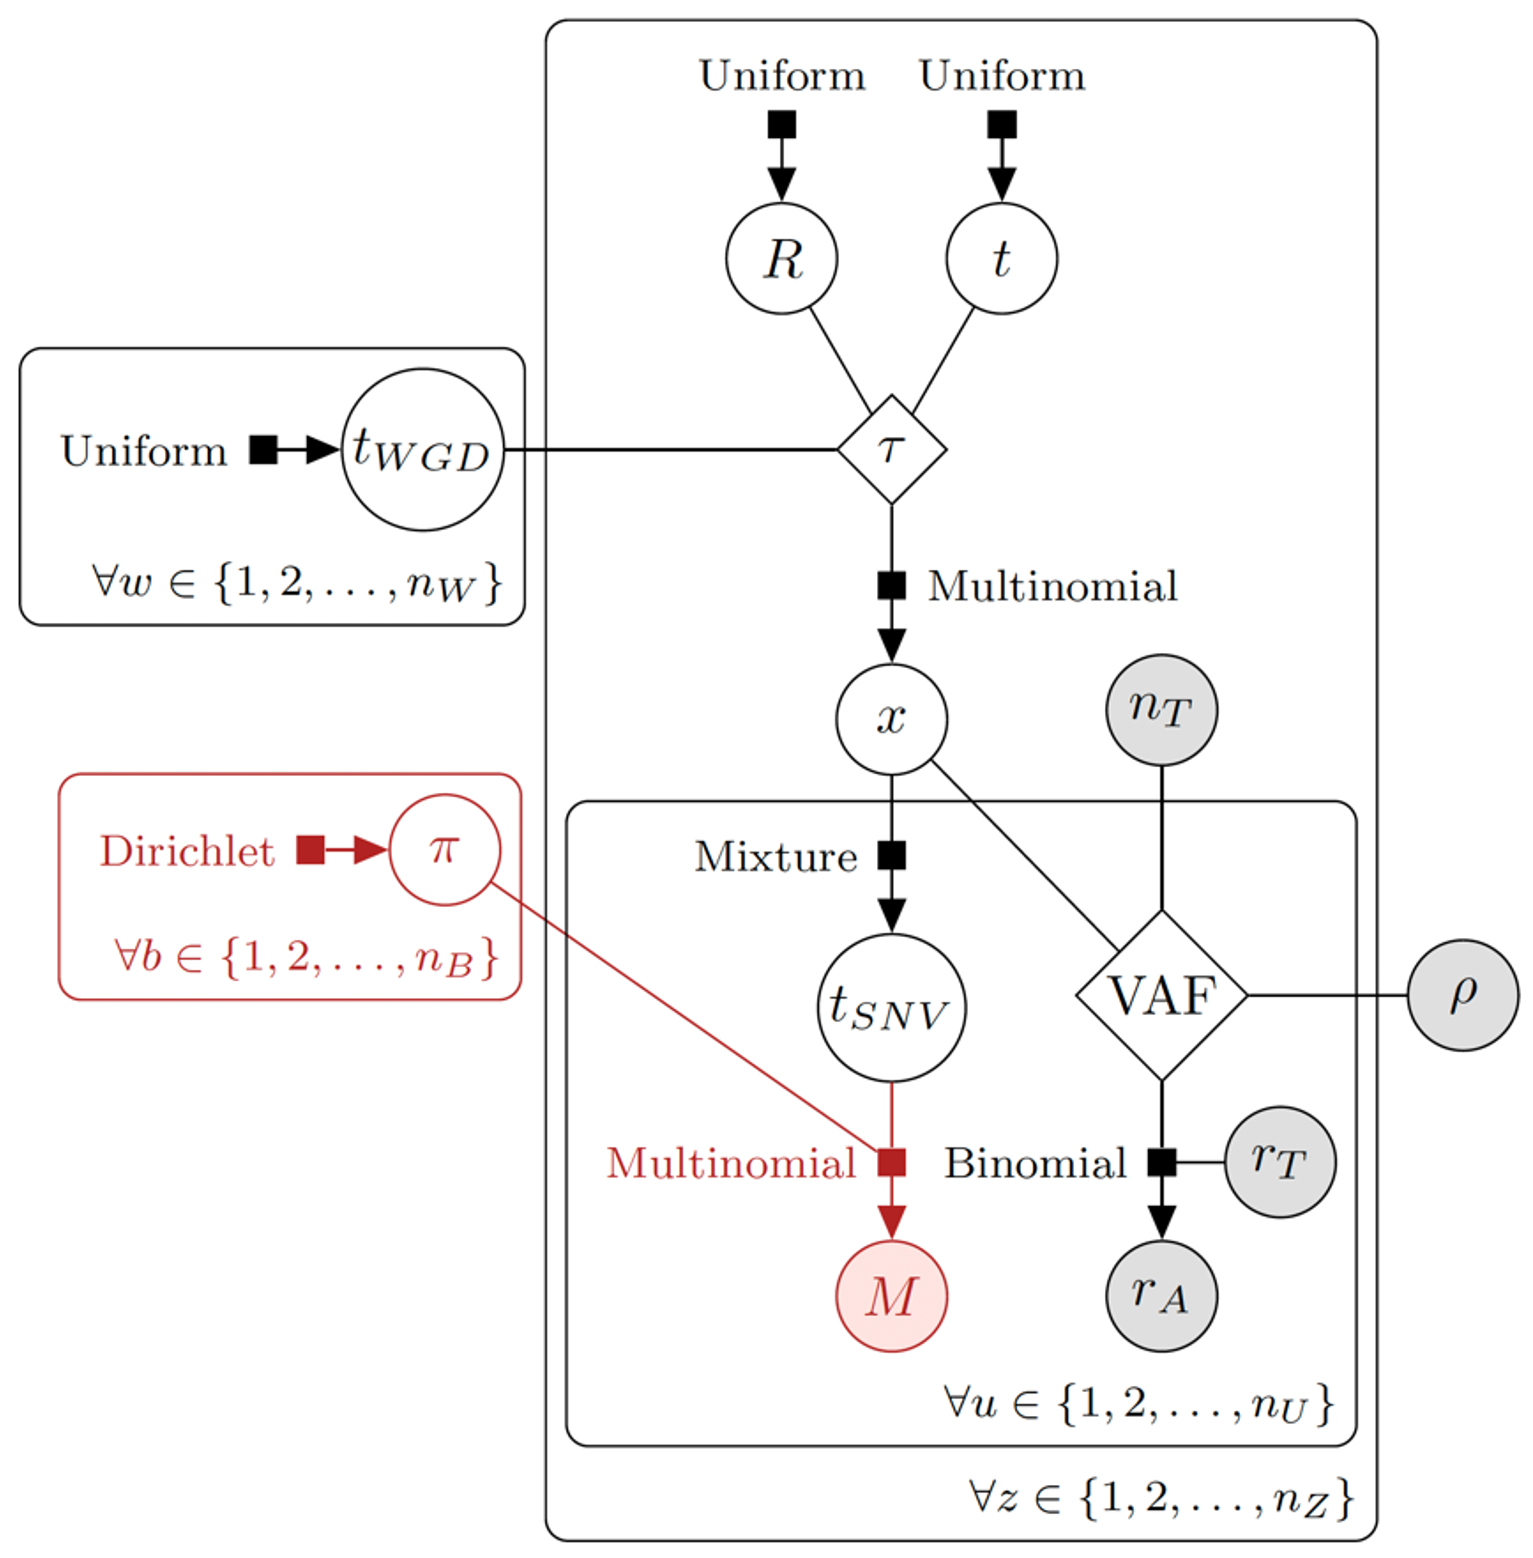
\includegraphics[width=2.5in]{./Figures/GRITIC_improvements.png}
  \caption{Improving the statistical power of GRITIC to determine the order of driver mutations. 
  Mutation signature timing (red) will both be added to GRITIC to improve gain and mutation timing precision. 
  In these probabilistic graphical models, data is represented by solid circles, probabilistic variables by empty circles, 
  deterministic variables by diamonds and probability distributions by solid squares.
}
  \label{GRITIC_improvements}
  \end{mdframed}
\end{wrapfigure}

\texttt{GRITIC} incorporates the timing of a single WGD but does not handle a second WGD event. 
Based on the work of Baker \textit{et al.}, we will update the \texttt{GRITIC} tool to include a second WGD event. 
This enhancement will improve the model’s ability to accurately capture the complex evolutionary history of cancer genomes.

\vspace{1em}
\noindent
By timing individual SNVs and leveraging the capabilities of \texttt{GRITIC}, 
we can align mutation timing with clonal copy number gains. 
Inputs such as mutational signature timing and the proportions of mutations at each clonal mutation multiplicity state will be crucial. 
improved precision timing data from 3.1 will inform Dirichlet prior distributions,
modeling mutation signature proportions over time to enhance accuracy (Fig.~\ref{GRITIC_improvements}).
%
%\vspace{1em}
%\noindent
%Variant allele frequency (VAF) of each SNV within a segment, determined by mutation multiplicity, tumor purity, and total tumor copy number, constrains SNV timing to overlap event tree edges with the same multiplicity, often resulting in broad ranges. 
Using temporally varying distributions of mutation signatures as priors will improve precision.

%\vspace{1em}
%\noindent
%We will extend \texttt{GRITIC} to estimate mutation signature proportions over mutation time. This involves discretizing mutation time into bins and mapping SNV timing to these bins to retrieve signature proportions. The sum over mutation signatures, weighted by their proportions in the corresponding bin, will provide the probability for any mutation based on context.

\vspace{1em}
\noindent
By jointly estimating mutation timing and time-series proportions of mutation signatures, 
we will integrate mutation signatures with gain route and timing, 
dramatically improving precision. 
This will enhance the temporal resolution of various driver mutations, 
including SNVs resulting in a gain or loss of function, 
benefiting individual tumor studies and enabling comprehensive analyses of 
cancer development pathways.

\paragraph{3.3. \SpecificAimThreeC}

Combine improvments to \texttt{GRITIC} from aims 3.1 and 3.2 into an accessible 
open-source software for use by the scientific community. 
To ensure the broad application of our improved precision mutation timing techniques, 
we will create user-friendly software tools. 
These tools will be made available as open-source software, 
accompanied by detailed documentation and tutorials to facilitate their use by other researchers in the field.

\paragraph{Challenges \& Alternative Approaches}

Developing improved precision mutation timing techniques poses several challenges, 
including the need for large and high-quality datasets, sophisticated computational models, and significant computational resources.
To address these challenges, we will collaborate with other research institutions to access extensive genomic datasets and leverage HPC resources. 
Additionally, we will employ rigorous validation techniques to ensure the accuracy and robustness of our methods. 
If initial approaches prove inadequate, we will explore alternative statistical models and computational frameworks to achieve our objectives. 
%Furthermore, ensuring the usability and accessibility of the developed software tools will 
%require careful consideration of user experience and extensive testing with a diverse group of researchers.


